% !TEX root = ../../main.tex

\subsection{An in-depth look at the NGA mechanism}%
\label{dut:indepth}

As it has been shown in the previous section, there are 
several avenues NGA tuning in the DUT-49 framework.
However, a fundamental understanding of the factors and 
energetics of the process itself may
lend itself to prediction of when the phenomenon occurs without 
experimental input, and even lead to the rational design of 
materials.

To this end, the adsorption of multiple probes was investigated 
at \SI{77}{\kelvin} with \textit{in situ} continuous low 
temperature microcalorimetry,
in order to observe the influence of the guest on the mechanism of
adsorption and NGA. In order to obtain a baseline of adsorption in 
the \textbf{op} phase, a non-flexible alternative is used. 
DUT-149 is the most similar material out of all previously studied
analogues, as it has the same linker length and nearly identical pore
size and surface area. 

Four gas probes were used, chosen as they 
have a non-trivial saturation pressure at this temperature: Ar,
\ce{N2}, \ce{CO} and \ce{O2}. Argon, as a 
noble gas, has a completely spherical molecule, which does not 
have any specific host-guest or guest-guest interactions. Nitrogen
is commonly used as the probe in material characterisation, 
and carries a weak quadrupole. Carbon monoxide has been used 
as it often forms coordination bonds through electron donation adducts.
Finally oxygen has an even stronger quadrupolar moment than 
nitrogen, which can interact with the surface in a similar way.
It is worth noting that both argon and carbon monoxide are below 
their freezing point at this temperature. \todo{check}

It should be mentioned that a large dataset was gathered
on these materials as experiments were performed with different 
amounts of sample, different gas introduction flowrates, as well as repeats
in identical conditions on samples which have undergone NGA. A list 
of experiments, as well as all isotherms and enthalpy curves measured can
be found in \autoref{appx:dut}.

\begin{figure}[p]
    \centering
    \begin{subfigure}{0.43\linewidth}
        \includegraphics[width=\linewidth]{ltc/dut-49-N2-log}%
        % \caption{}\label{dut:fgr:dut-48-prop-log}
    \end{subfigure}%
    \begin{subfigure}{0.43\linewidth}
        \includegraphics[width=\linewidth]{ltc/dut-149-N2-log}%
        % \caption{}\label{dut:fgr:dut-48-prop-enth}
    \end{subfigure}%

    \begin{subfigure}{0.43\linewidth}
        \includegraphics[width=\linewidth]{ltc/dut-49-N2-enth}%
        % \caption{}\label{dut:fgr:dut-48-prop-log}
    \end{subfigure}%
    \begin{subfigure}{0.43\linewidth}
        \includegraphics[width=\linewidth]{ltc/dut-149-N2-enth}%
        % \caption{}\label{dut:fgr:dut-48-prop-enth}
    \end{subfigure}%

    \begin{subfigure}{0.43\linewidth}
        \includegraphics[width=\linewidth]{ltc/dut-49-CO-log}%
        % \caption{}\label{dut:fgr:dut-48-prop-log}
    \end{subfigure}%
    \begin{subfigure}{0.43\linewidth}
        \includegraphics[width=\linewidth]{ltc/dut-149-CO-log}%
        % \caption{}\label{dut:fgr:dut-48-prop-enth}
    \end{subfigure}%

    \begin{subfigure}{0.43\linewidth}
        \includegraphics[width=\linewidth]{ltc/dut-49-CO-enth}%
        % \caption{}\label{dut:fgr:dut-48-prop-log}
    \end{subfigure}%
    \begin{subfigure}{0.43\linewidth}
        \includegraphics[width=\linewidth]{ltc/dut-149-CO-enth}%
        % \caption{}\label{dut:fgr:dut-48-prop-enth}
    \end{subfigure}%

    \caption{}%
    \label{dut:fgr:dut-ltc-comp1}
\end{figure}

The isotherms and the corresponding enthalpy curves for both 
DUT-49 and DUT-149 are shown in \autoref{dut:fgr:dut-ltc-comp1}
for \ce{N2} and \ce{CO} and in \autoref{dut:fgr:dut-ltc-comp2}
for \ce{Ar} and \ce{O2}. A cursory observation of the isotherms
reveals that the DUT-149 framework is not as stiff as 
previously assumed. A clear NGA step can be found in the 
oxygen isotherm, suggesting that adsorption of this probe is capable 
of overcoming the higher energy barrier of linker buckling in 
this methyl functionalised version.
If comparing the isotherms measured on the two materials, they
are seen to be nearly identical until structural contraction.
The total amount adsorbed after pore re-opening is also in a 
2\% range with all probes. The assumption that the mechanism 
of adsorption in DUT-49 can be likened to its functionalised
version holds in this case.

Another surprising behaviour
can be seen in the nitrogen isotherm on DUT-49. While an NGA
discontinuity is still present, structural re-opening takes
place in several distinct steps. This behaviour in in
agreement with the study published by
 \citet{krauseEffectCrystalliteSize2018}
on the evolution of the contraction step with variation of 
crystallite size. In their paper, the increase of average 
crystal dimensions is seen to evolve the structure from non-flexible 
to a progressively better defined NGA transition. \textit{In situ} 
PXRD shows that between complete structural stiffness and a 
purely \textbf{op/cp} phase transition, several intermediate 
pore forms can be accessed. It can therefore be theorised that 
nitrogen adsorption takes place near the lower limit of 
favourable transition energetics, where particulate surface 
effects can have a high influence on the stability domain of
each phase.

If focusing on the pore filling behaviour of DUT-149, two types
of steps can be seen. While the initial part of the isotherm 
(below \(0.1~p/p_0\)) is typical of BET-type multilayer adsorption
with a possible micropore filling step at very low pressure,
the large framework pores are seen to be filled in either a single or
two-step process.
Both nitrogen and carbon monoxide have two distinct filling
steps, corresponding to the octahedral and tetrahedral pores,
respectively. The two steps are accompanied by identical 
peaks in the enthalpy curve. This points to a highly similar 
filling process for both pores, with cooperative adsorption
dominating the pore filling mechanism, rather than guest-host 
effects. The argon isotherm, similar to the behaviour of 
butane at \SI{303}{\kelvin}, shows a very sharp single-step process,
which can be likened to condensation in a mesopore. As the 
two pores in the DUT-49/149 framework are interconnected through 
windows of \(\approx\)\SI{1}{\nano\metre}, pore filling 
in one type of pore can induce filling in the adjacent pore of 
a larger size. The sudden transition to the fluid phase can further
be understood if considering the MOF pores are nearly mesoscale in 
length. Adsorption in such pores can be characterised through 
the formation of a vapour-like spinodal if the pore size is within
a ``critical hysteresis radius''~\cite{hiratsukaCriticalEnergyBarrier2016}.
\todo{window size}

\begin{figure}[p]
    \centering

    \begin{subfigure}{0.43\linewidth}
        \includegraphics[width=\linewidth]{ltc/dut-49-Ar-log}%
        % \caption{}\label{dut:fgr:dut-48-prop-log}
    \end{subfigure}%
    \begin{subfigure}{0.43\linewidth}
        \includegraphics[width=\linewidth]{ltc/dut-149-Ar-log}%
        % \caption{}\label{dut:fgr:dut-48-prop-enth}
    \end{subfigure}%

    \begin{subfigure}{0.43\linewidth}
        \includegraphics[width=\linewidth]{ltc/dut-49-Ar-enth}%
        % \caption{}\label{dut:fgr:dut-48-prop-log}
    \end{subfigure}%
    \begin{subfigure}{0.43\linewidth}
        \includegraphics[width=\linewidth]{ltc/dut-149-Ar-enth}%
        % \caption{}\label{dut:fgr:dut-48-prop-enth}
    \end{subfigure}%

    \begin{subfigure}{0.43\linewidth}
        \includegraphics[width=\linewidth]{ltc/dut-49-O2-log}%
        % \caption{}\label{dut:fgr:dut-48-prop-log}
    \end{subfigure}%
    \begin{subfigure}{0.43\linewidth}
        \includegraphics[width=\linewidth]{ltc/dut-149-O2-log}%
        % \caption{}\label{dut:fgr:dut-48-prop-enth}
    \end{subfigure}%

    \begin{subfigure}{0.43\linewidth}
        \includegraphics[width=\linewidth]{ltc/dut-49-O2-enth}%
        % \caption{}\label{dut:fgr:dut-48-prop-log}
    \end{subfigure}%
    \begin{subfigure}{0.43\linewidth}
        \includegraphics[width=\linewidth]{ltc/dut-149-O2-enth}%
        % \caption{}\label{dut:fgr:dut-48-prop-enth}
    \end{subfigure}%

    \caption{}%
    \label{dut:fgr:dut-ltc-comp2}
\end{figure}

A common feature to almost all measured isotherms is the identical
adsorption mechanism before pore size effects come into play.
Indeed if enthalpy curves recorded with different adsorbates, at different
temperatures and even on different DUT analogues are compared at low 
loading, they may be mistaken for the same data.
This typical enthalpy curve starts at relatively low values compared 
to adsorption in the same conditions on a similar paddlewheel based 
MOF such as HKUST-1, then increases to a local maxima followed
by a gentle downward slope.
This feature is typical of cooperative adsorption, and suggests that
the interactions with the framework are generally low. The only 
exception to this case are adsorbates which can act with the 
Cu paddlewheel in some way, either through adduct formation, 
electron donation or \(\pi\) backbonding interactions. 


\begin{figure}[htb]
    \centering
    \begin{subfigure}{0.5\linewidth}
        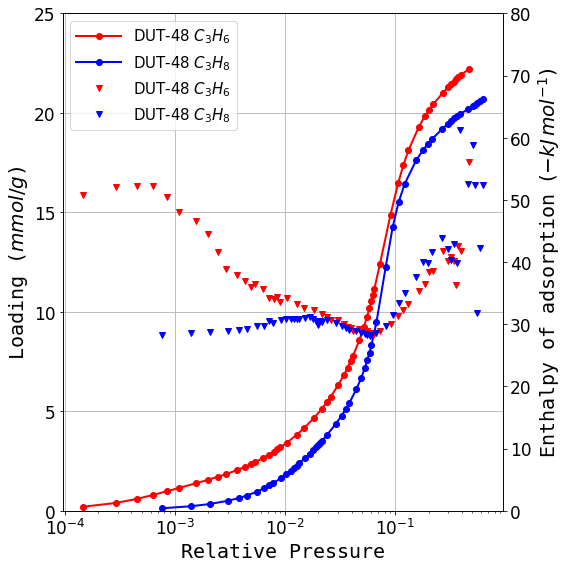
\includegraphics[width=\linewidth]{butane/dut-48-prop-log}%
        \caption{}\label{dut:fgr:dut-48-prop-log}
    \end{subfigure}%
    \begin{subfigure}{0.5\linewidth}
        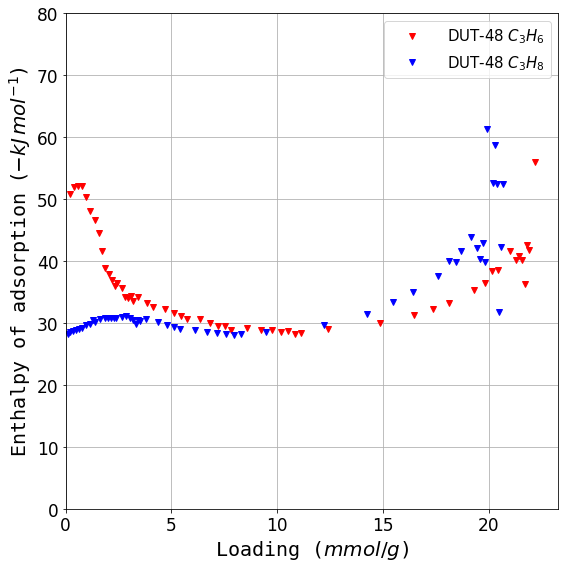
\includegraphics[width=\linewidth]{butane/dut-48-prop-enth}%
        \caption{}\label{dut:fgr:dut-48-prop-enth}
    \end{subfigure}%
    \caption{The (a) isotherms and (b) enthalpy curves of propane 
    and propylene adsorption on DUT-48, highlighting the high energy
    of \ce{C3H6} on specific sites at low pressure, likely to be 
    \(\pi\)-Cu interactions.}%
    \label{dut:fgr:dut-48-prop}
\end{figure}